% Native editable composition from verified, unchanged IDE images.
\par
\begin{figure}[htbp]
\centering
\sbox0{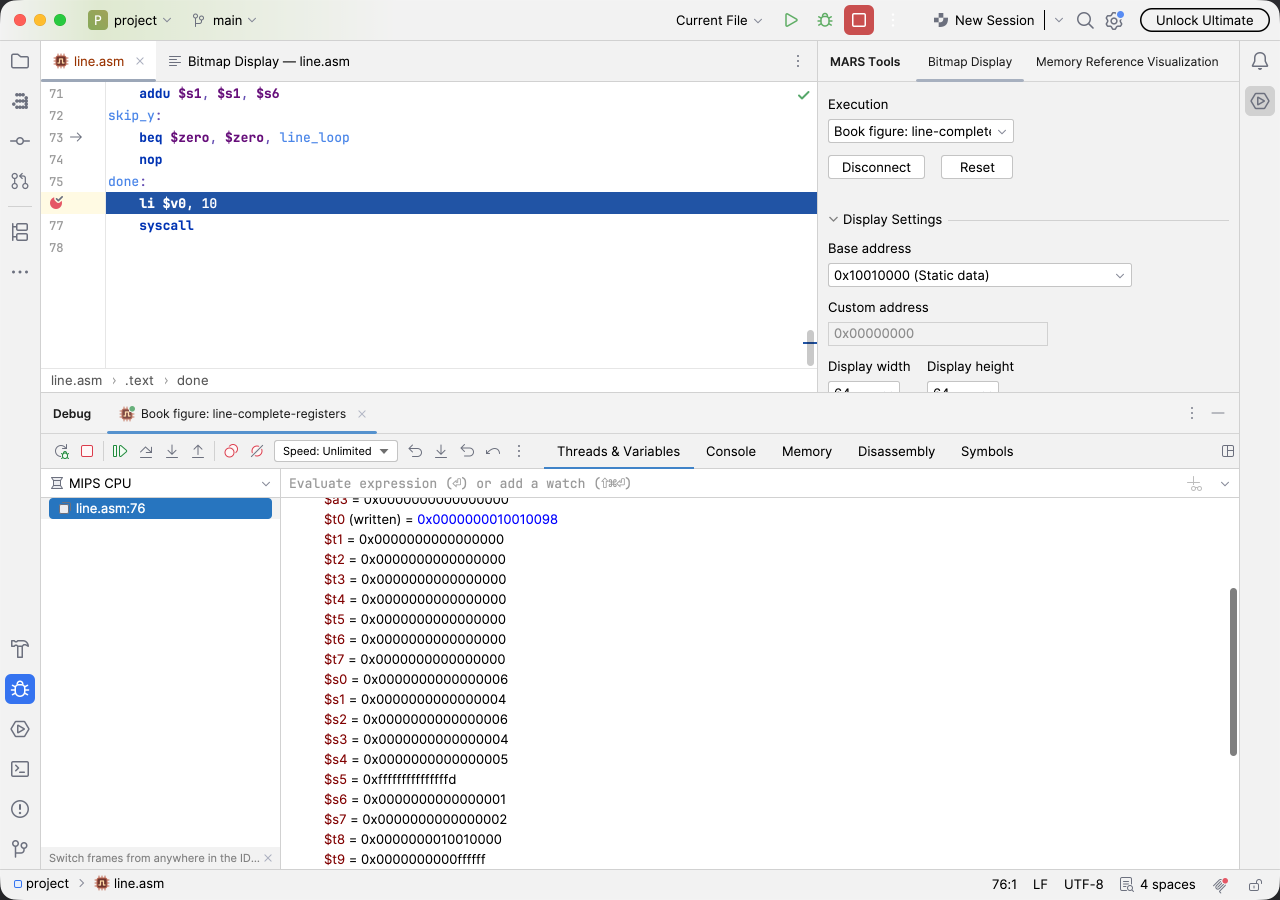
\includegraphics[artifact]{book/captures/007-bresenham-line/f04-complete/registers.png}}
\sbox2{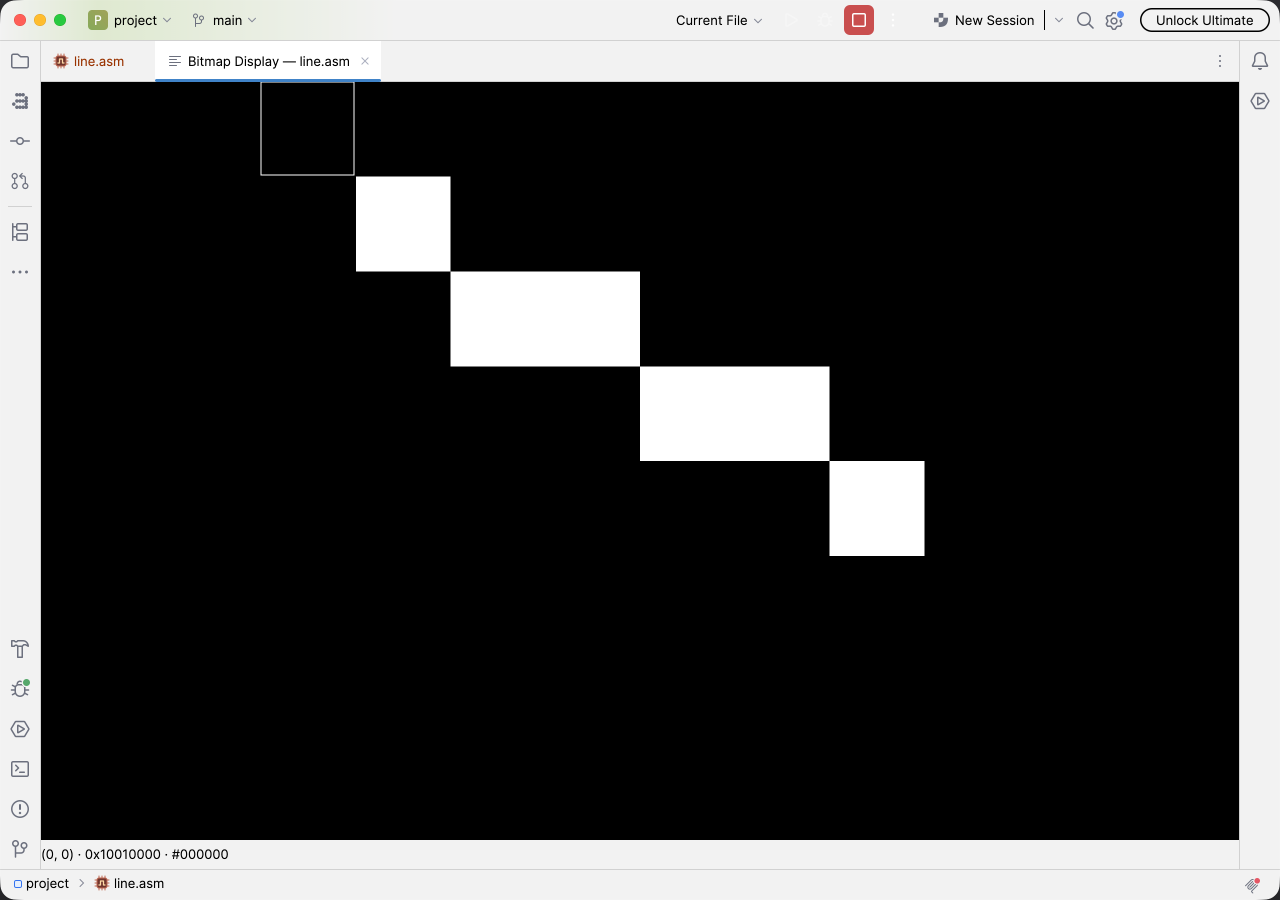
\includegraphics[artifact]{book/captures/007-bresenham-line/f04-complete/bitmap.png}}
\edef\MARScompletesourceLeft{\the\dimexpr0.036718750\wd0\relax}
\edef\MARScompletesourceBottom{\the\dimexpr0.757777778\ht0\relax}
\edef\MARScompletesourceRight{\the\dimexpr0.611718750\wd0\relax}
\edef\MARScompletesourceTop{\the\dimexpr0.164444444\ht0\relax}
\edef\MARScompletestateLeft{\the\dimexpr0.246093750\wd0\relax}
\edef\MARScompletestateBottom{\the\dimexpr0.075555556\ht0\relax}
\edef\MARScompletestateRight{\the\dimexpr0.596875000\wd0\relax}
\edef\MARScompletestateTop{\the\dimexpr0.740000000\ht0\relax}
\edef\MARScompleteplotLeft{\the\dimexpr0.203906250\wd2\relax}
\edef\MARScompleteplotBottom{\the\dimexpr0.066666667\ht2\relax}
\edef\MARScompleteplotRight{\the\dimexpr0.203906250\wd2\relax}
\edef\MARScompleteplotTop{\the\dimexpr0.091111111\ht2\relax}
\edef\MARScompletesavedLeft{\the\dimexpr0.246093750\wd0\relax}
\edef\MARScompletesavedBottom{\the\dimexpr0.364444444\ht0\relax}
\edef\MARScompletesavedRight{\the\dimexpr0.599218750\wd0\relax}
\edef\MARScompletesavedTop{\the\dimexpr0.606666667\ht0\relax}
\begin{tikzpicture}[alt={Four annotated details at done before exit service ten is selected. The working coordinate is six four and the running error is two. The original bitmap contains exactly six white cells: one one, two two, three two, four three, five three and six four. Scratch register t2 still contains zero from the previous update.}]
\node[anchor=north west,inner sep=0,font=\small\bfseries] (source-title) at (6mm,0) {The endpoint has been painted and recognized};
\node[anchor=north west,inner sep=0] (source) at ([yshift=-1mm]source-title.south west) {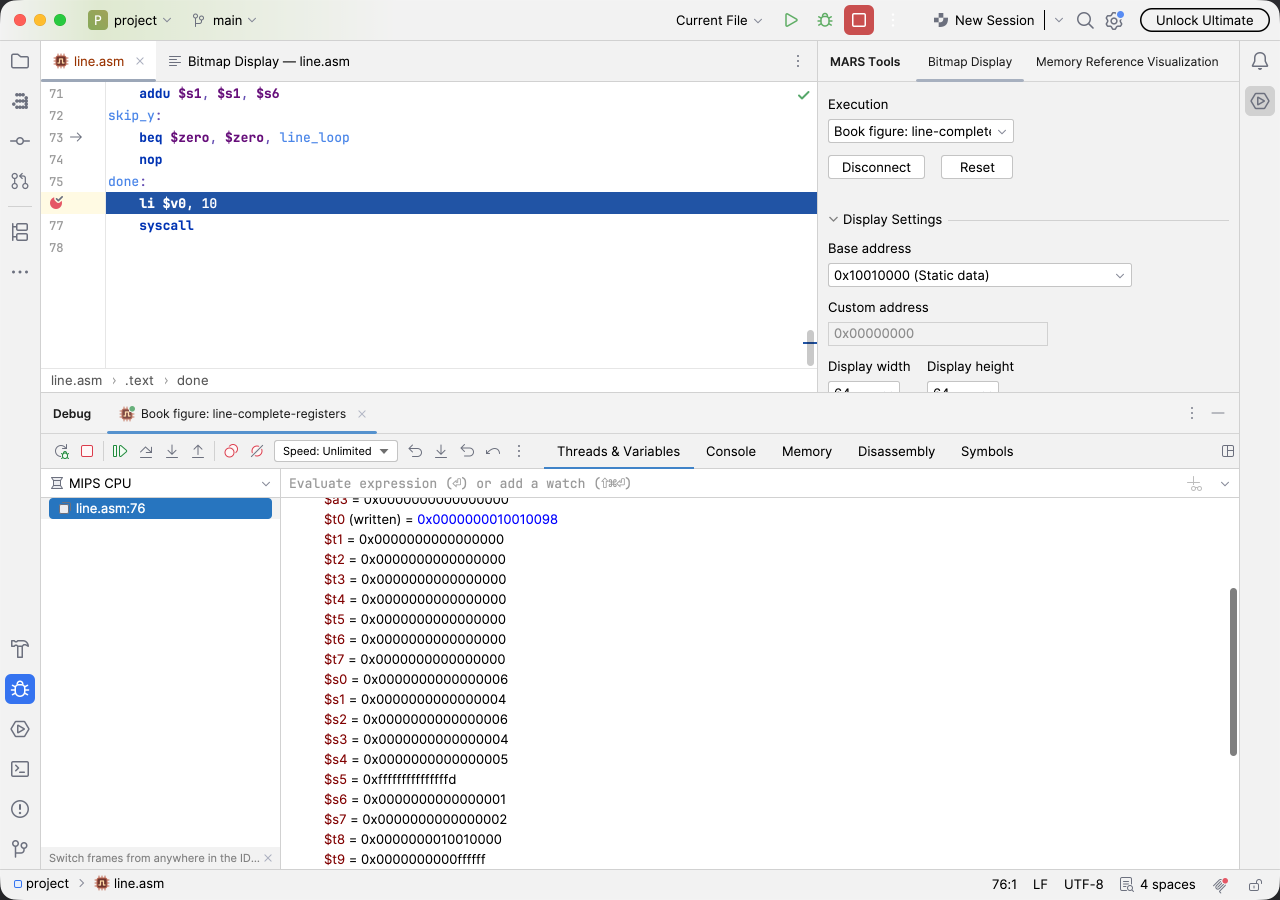
\includegraphics[width=0.7\linewidth,artifact,trim={\MARScompletesourceLeft{} \MARScompletesourceBottom{} \MARScompletesourceRight{} \MARScompletesourceTop{}},clip]{book/captures/007-bresenham-line/f04-complete/registers.png}};
\begin{scope}[shift={(source.south west)},x={($(source.south east)-(source.south west)$)},y={($(source.north west)-(source.south west)$)}]
\draw[black,line width=0.7pt] (0.135555556,0.057142857) rectangle (0.377777778,0.371428571);
\node[draw=black,fill=white,circle,inner sep=1.5pt,font=\footnotesize] at ($(0.135555556,0.371428571)+(-3mm,0)$) {1};
\end{scope}
\node[anchor=north west,inner sep=0,font=\small\bfseries] (state-title) at ([yshift=-2mm]source.south west) {The working coordinate equals the endpoint};
\node[anchor=north west,inner sep=0] (state) at ([yshift=-1mm]state-title.south west) {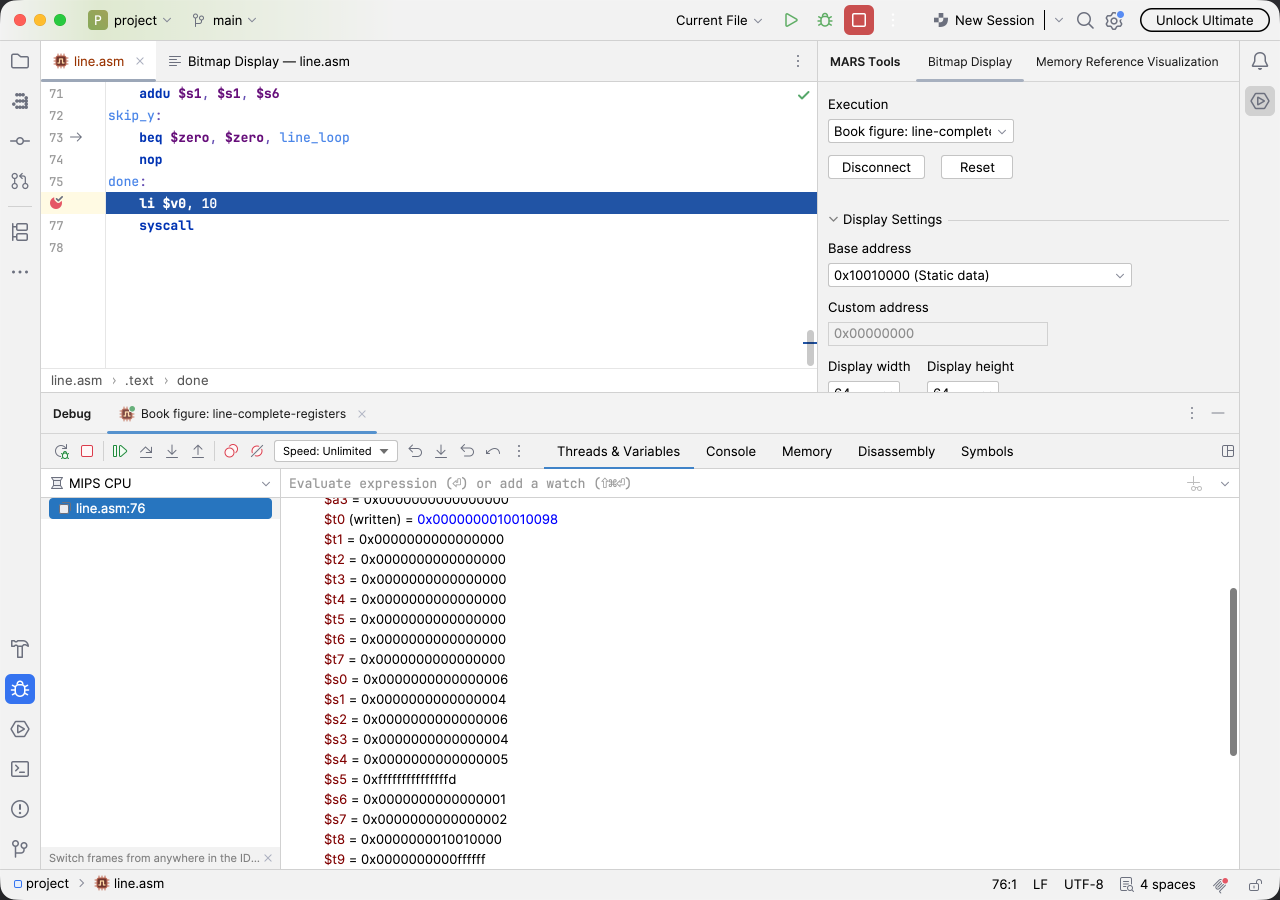
\includegraphics[width=0.4\linewidth,artifact,trim={\MARScompletestateLeft{} \MARScompletestateBottom{} \MARScompletestateRight{} \MARScompletestateTop{}},clip]{book/captures/007-bresenham-line/f04-complete/registers.png}};
\begin{scope}[shift={(state.south west)},x={($(state.south east)-(state.south west)$)},y={($(state.north west)-(state.south west)$)}]
\draw[black,line width=0.7pt] (0.029850746,0.018072289) rectangle (0.970149254,0.981927711);
\node[draw=black,fill=white,circle,inner sep=1.5pt,font=\footnotesize] at ($(0.029850746,0.981927711)+(-3mm,0)$) {2};
\end{scope}
\node[anchor=north west,inner sep=0,font=\small\bfseries] (plot-title) at ([xshift=0.49\linewidth]state-title.north west) {Both endpoints are included};
\node[anchor=north west,inner sep=0] (plot) at ([yshift=-1mm]plot-title.south west) {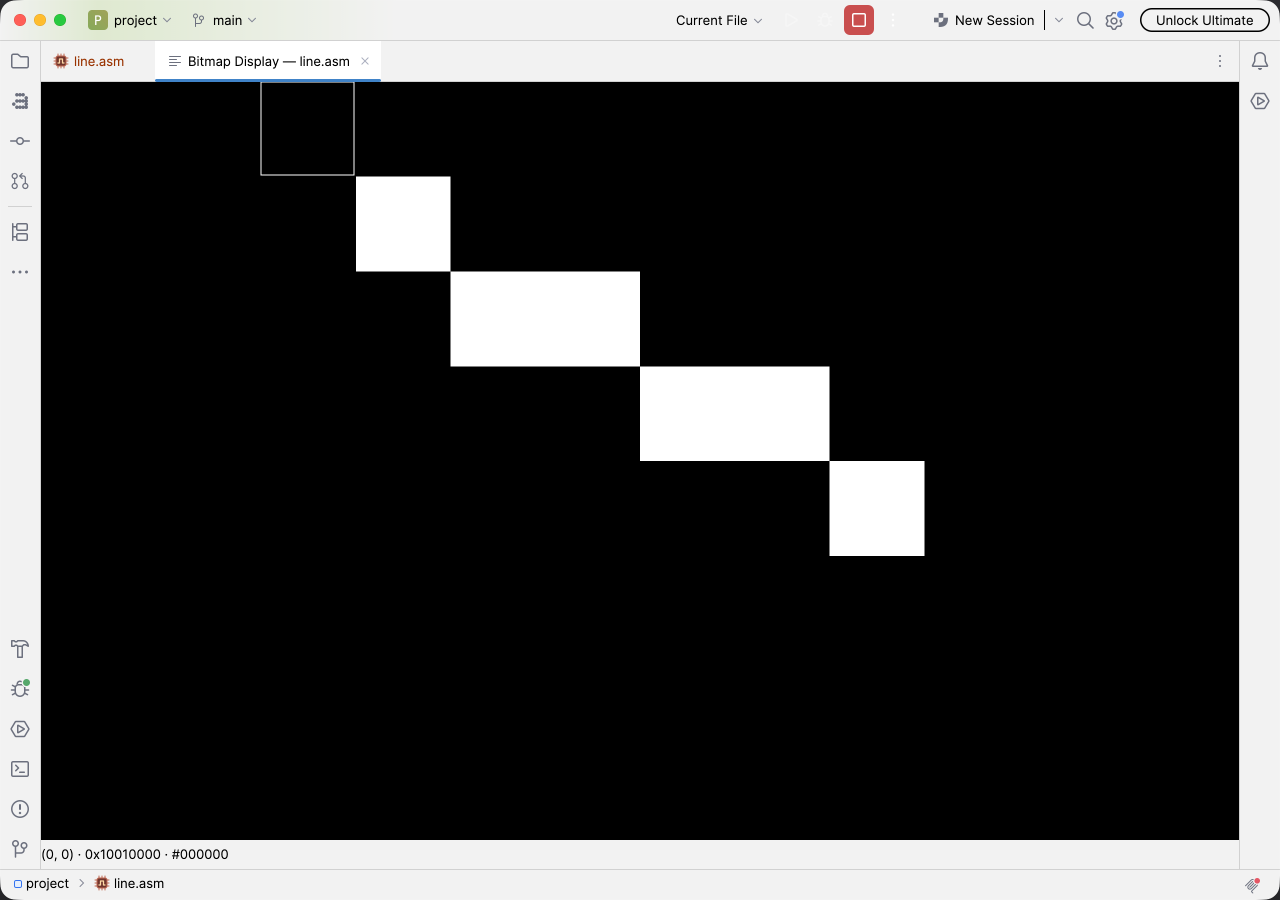
\includegraphics[width=0.32\linewidth,artifact,trim={\MARScompleteplotLeft{} \MARScompleteplotBottom{} \MARScompleteplotRight{} \MARScompleteplotTop{}},clip]{book/captures/007-bresenham-line/f04-complete/bitmap.png}};
\begin{scope}[shift={(plot.south west)},x={($(plot.south east)-(plot.south west)$)},y={($(plot.north west)-(plot.south west)$)}]
\draw[black,line width=0.7pt] (0.000000000,0.000000000) rectangle (1.000000000,1.000000000);
\node[draw=black,fill=white,circle,inner sep=1.5pt,font=\footnotesize] at ($(0.000000000,1.000000000)+(-3mm,0)$) {3};
\foreach \c in {0,...,7} {\node[anchor=north,font=\scriptsize,inner sep=0] at ({(\c+0.5)/8},-0.035) {\c}; \node[anchor=east,font=\scriptsize,inner sep=0] at (-0.025,{1-(\c+0.5)/8}) {\c};}
\node[anchor=north,font=\scriptsize,inner sep=0] at (0.5,-0.11) {$x$}; \node[anchor=east,font=\scriptsize,inner sep=0] at (-0.10,0.5) {$y$};
\end{scope}
\node[anchor=north west,inner sep=0,font=\small\bfseries] (saved-title) at ([yshift=-2mm]state.south west) {No doubled error was evaluated for the endpoint};
\node[anchor=north west,inner sep=0] (saved) at ([yshift=-1mm]saved-title.south west) {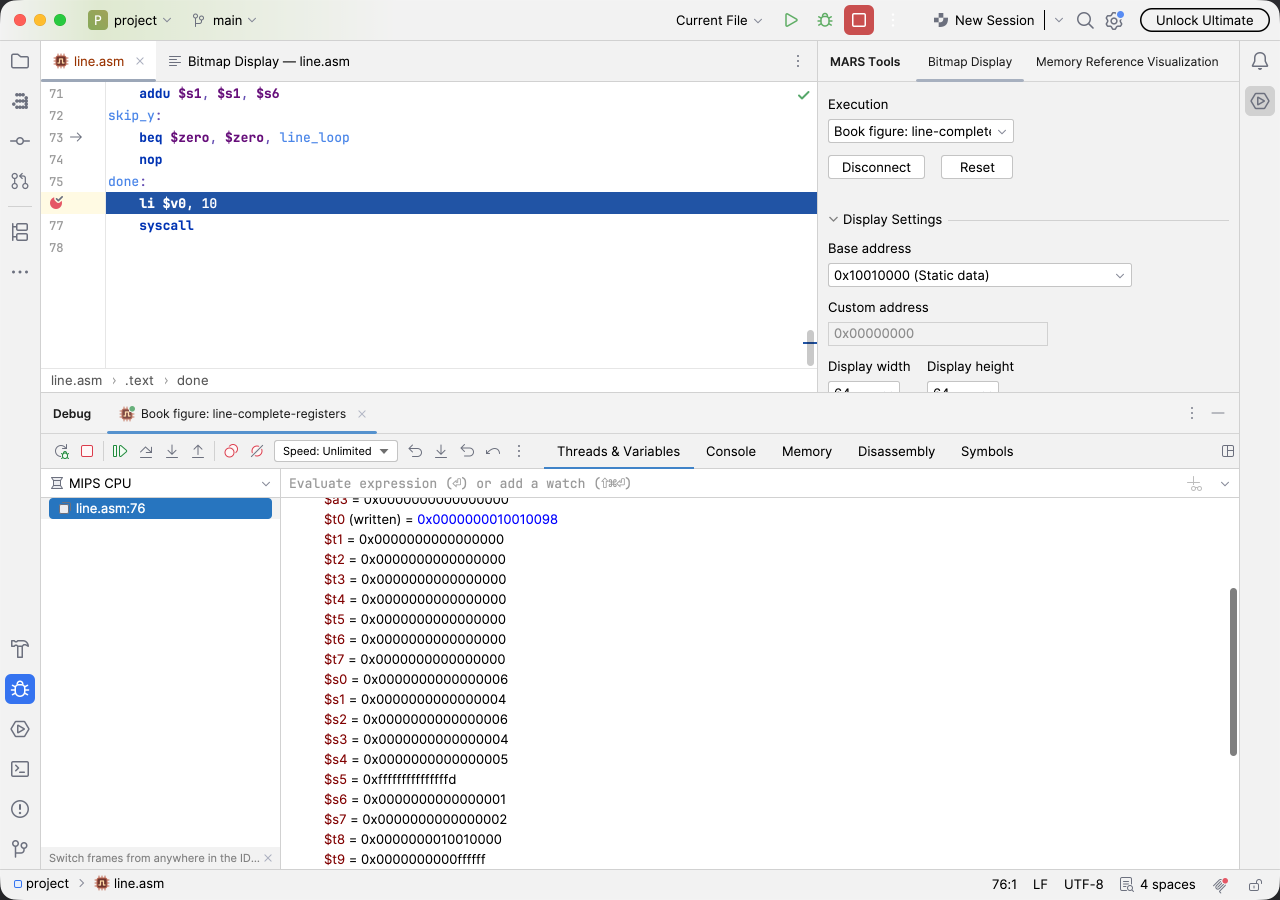
\includegraphics[width=0.4\linewidth,artifact,trim={\MARScompletesavedLeft{} \MARScompletesavedBottom{} \MARScompletesavedRight{} \MARScompletesavedTop{}},clip]{book/captures/007-bresenham-line/f04-complete/registers.png}};
\begin{scope}[shift={(saved.south west)},x={($(saved.south east)-(saved.south west)$)},y={($(saved.north west)-(saved.south west)$)}]
\draw[black,line width=0.7pt] (0.030303030,0.115384615) rectangle (0.969696970,0.884615385);
\node[draw=black,fill=white,circle,inner sep=1.5pt,font=\footnotesize] at ($(0.030303030,0.884615385)+(-3mm,0)$) {4};
\end{scope}
\end{tikzpicture}
\par\smallskip
\begin{minipage}{\linewidth}
\small
\begin{enumerate}
\item The next \texttt{li \$v0, 10} begins normal exit. The last pixel store and both endpoint comparisons have completed. Control reached \texttt{done} before another coordinate update.
\item The working coordinate is $(6,4)$ and the running error is 2. The last cell\textquotesingle s address is \texttt{0x10010000}+ $4(8\cdot4+6)$ = \texttt{0x10010098}. Neither coordinate needs another increment.
\item The white cells are $(1,1)$, $(2,2)$, $(3,2)$, $(4,3)$, $(5,3)$ and $(6,4)$. Exactly six word stores produced this overlay. The other 58 words keep their initial zeros; the program does not clear the framebuffer. The checks also preserve every input and guard.
\item \texttt{\$t2}=0 remains from the update after $(5,3)$, when the running error was zero. It is not a newly calculated value for $(6,4)$. The endpoint path bypasses the next \texttt{sll}, so there is no reason to evaluate $2\cdot2$ before exiting.
\end{enumerate}
\end{minipage}
\caption{Six cells form the completed overlay before exit. The endpoint test bypassed another error update.}
\label{capture:007-bresenham-line-f04-complete}
\end{figure}
\par
